%*********************************************************************************************************
% Modified Project from PAGSA's UVic Thesis Template: https://github.com/PAGSA/UVic-latex-thesis-template
% Development Credit for PAGSA's UVic Thesis Template: Caleb Miller
% 
% Designed by Samuel Fielder
%
% Notes:
% Developed in preparation for the March 2024 Software Plumbing Workshop
% See README.md for more information regarding the structure for this astronomy-specific project
%*********************************************************************************************************

%*********************************************************************************************************
% PACKAGES AND DEFINTIONS
%*********************************************************************************************************
\documentclass[12pt,oneside]{book}
\pagestyle{headings}

% Note that the line below could be modified to suit a
% particular system since the "geometry" package behaves
% differently in Unix, Windows and Mac, especially for the
% top margins.
% Adjust the parameter "top" (measuring the height of the
% space allocated to a header) and "headsep" (measuring
% the distance from the bottom of the header to the
% first line of text.
\usepackage[top=1.3in,left=1in,bottom=1in,right=1in,headsep=0.5in]{geometry}

\usepackage{setspace}
\onehalfspacing
%\doublespacing

% Headers and footers for thesis
\usepackage{fancyhdr}

\markboth{}{}
\newcommand\startchapter[1]{\chapter{#1}\thispagestyle{myheadings}}
\newcommand\startappendix[1]{\chapter{#1}\thispagestyle{myheadings}}
\newcommand\startfirstchapter[1]{\chapter{#1}}

% Manual addition of section to Table of Contents
\newcommand\TOCadd[1]{\newpage\phantomsection\addcontentsline{toc}{chapter}{#1}}

% Float Customization
\renewcommand{\floatpagefraction}{0.01}

% Customization of Tables of Contents and List of Figures/Tables
\usepackage{tocloft}
\renewcommand\cfttabpresnum{Table\ }
\renewcommand\cfttabnumwidth{0.75in}
\renewcommand\cftfigpresnum{Figure\ }
\renewcommand\cftfignumwidth{0.80in}
\newcommand{\HRule}{\rule{\linewidth}{0.5mm}}
 % sets packages to use for thesis style implementation
% packages

% dvipsnames, svgnames - were included in the documentclass call

\usepackage{amsmath}
\usepackage{amsthm}
\usepackage{amssymb}

% HEADINGS
%*********************************************************************************************************
% This changes the headings go that they are prettier, this can be commented out for traditional headings.
\usepackage{sectsty}
\allsectionsfont{\bfseries}% set all the section font to bfseries
\chapterfont{\centering\Large} % set the sizes of chapters, sections ...
\sectionfont{\normalsize}
\subsectionfont{\normalsize}

\usepackage{xspace}

\usepackage{verbatim}

\usepackage{graphics}
\usepackage{graphicx}

\usepackage{layout}
\usepackage{changebar}
\usepackage{pdfpages}
\usepackage{geometry}
\usepackage[export]{adjustbox}[2011/08/13]
\usepackage{notoccite}

\usepackage{caption}
\usepackage{subcaption}

\usepackage{varioref}

\usepackage{url}

\usepackage{natbib}
\usepackage{aastex_hack}

% HYPERLINKS (must be last to work properly, caution with other packages)
%*************************************************************************************************************
\usepackage{hyperref}
\hypersetup{
	colorlinks,
	linkcolor=blue,
	linktocpage=true,
	citecolor=blue,
	urlcolor=olive
}
 % sets other packages for users to use

% inclusion of table-related packages
\usepackage{xltabular}
\usepackage{threeparttablex}
\usepackage{booktabs, caption}
\usepackage{multirow}
\usepackage{pdflscape}

%*********************************************************************************************************
% PACKAGES ONLY USED FOR EXAMPLE PDF - CODE LISTINGS
% if code listings aren't required, delete this section
%*********************************************************************************************************
\usepackage{listings, xcolor}
\definecolor{backcolour}{rgb}{0.95,0.95,0.95}
\definecolor{codegreen}{rgb}{0,0.6,0}

% Define a custom style
\lstdefinestyle{CustomStyle}{
    backgroundcolor=\color{backcolour},   
    commentstyle=\color{codegreen},
    basicstyle=\ttfamily\footnotesize,
    breakatwhitespace=false,         
    breaklines=true,                 
    keepspaces=true,                 
    numbers=left,       
    numbersep=5pt,                  
    showspaces=false,                
    showstringspaces=false,
    showtabs=false,                  
    tabsize=2,
}
\lstset{style=CustomStyle}
%*********************************************************************************************************


% can optionally set a graphics path
\graphicspath{{content/figures/}}

% the following line stops footnotes from splitting onto two pages
\interfootnotelinepenalty=10000

%*********************************************************************************************************
% INCLUDE ONLY
%*********************************************************************************************************
% allows compiling of individual chapters for faster compile times (useful for speedy format checking)

% \includeonly{chapters/7/coolstuff}

%*********************************************************************************************************
% DOCUMENT
%*********************************************************************************************************
\begin{document}

    % choose one of the following lines, not both
    \newcommand{\PhDorMas}{Thesis }
\newcommand{\PhDorMaster}{MASTER OF SCIENCE} % sets up the document for a Masters thesis
    % \newcommand{\PhDorMas}{Dissertation }
\newcommand{\PhDorMaster}{DOCTOR OF PHILOSOPHY} % sets up the document for a PhD thesis

    %*****************************************************************
% SETUP
%**********************************************************************
\newcommand{\yourname}{A Hopeful Graduate: Samuel Fielder}
\newcommand{\thesistitle}{An Example Thesis Made With \LaTeX \ for Astronomy Students}
% one needs to make adjustments for a Master's Thesis
\newcommand\nameanddegrees{%
\yourname\\
B.Sc., University of WhoKnowsWhere, 2053\\
M.Sc., University of AnotherOne, 2054}
\newcommand\panel{%
\\\panelist{Dr. R.\ Supervisor Main}{Supervisor}{Department of Same As Candidate}
\\\panelist{Dr. M.\ Member One}{Departmental Member}{Department of Same As Candidate}
\\\panelist{Dr. Member Two}{Departmental Member}{Department of Same As Candidate}
\\\panelist{Dr. Outside Member}{Outside Member}{Department of Not Same As Candidate}}
%\HRule\\\panelist{Dr. \Ans{Current Unknown}}{Additional Member}{Department of \Ans{Current Unknown Department}}}

%*************************************************************************************************
% SET INITIAL STYLES
%*************************************************************************************************
\newcommand\tpbreak{\\[\baselineskip]} % titlepage break

\newpage
\thispagestyle{empty} % suppress numbers on the first page

% setting header and footer values
\pagestyle{myheadings}
\pagenumbering{roman}
% We use this in addition to the default \LaTeX page configuration routines
% because we have no way of saying \thispagestyle after the glossary and bibliography starts.
\fancypagestyle{plain}{%
\fancyhf{}
\fancyhead[R]{\thepage}
\renewcommand{\headrulewidth}{0pt}
\renewcommand{\footrulewidth}{0pt}
}

%*************************************************************************************************
% TITLE PAGES
%*************************************************************************************************
\input frontmatter/titlepage % title page
\input frontmatter/committee % supervisory commitee

%*************************************************************************************************
% ABSTACT
%*************************************************************************************************
\input frontmatter/abstract

\renewcommand{\contentsname}{\large\textbf{Table of Contents}}
\TOCadd{Table of Contents}\tableofcontents
\renewcommand{\listtablename}{\large\textbf{List of Tables}}
\TOCadd{List of Tables}\listoftables
\setcounter{lofdepth}{2}
\renewcommand{\listfigurename}{\large\textbf{List of Figures}}
\TOCadd{List of Figures}\listoffigures

%*************************************************************************************************
% GLOSSARY
%*************************************************************************************************
% the following lines need to be uncommented if you are using a glossary
% see https://github.com/PAGSA/UVic-latex-thesis-template for glossary implementation
% \newpage
% \glsaddall     
% \printglossaries 
% \printglossary[title={List of Symbols}] %Use this instead of printglossaries if you want a different title

%*************************************************************************************************
% ACKNOWLEDGEMENTS
%*************************************************************************************************
\input frontmatter/acknowledgements

%*************************************************************************************************
% DEDICATIONS
%*************************************************************************************************
\input frontmatter/dedications

%*************************************************************************************************
% HEADER AND FOOTER SETUP
%*************************************************************************************************
\newpage
\pagestyle{myheadings}
\pagenumbering{arabic}
% We use this in addition to the default LaTeX page configuration routines
% because we have no way of saying \thispagestyle after the bibliography starts.
\fancypagestyle{plain}{%
\fancyhf{}
\fancyhead[R]{\ifnum\thepage=1\relax\else\thepage\fi}
\renewcommand{\headrulewidth}{0pt}
\renewcommand{\footrulewidth}{0pt}
}
 % inserts the frontmatter 

    \newpage

    % include the content of the thesis
    \startfirstchapter{Introduction}
\label{sec: intro}

The main goal of this AstroExample PDF, is to give an overview of what this template thesis will look like to the user. Additionally, the different sections contained within give specific examples of how to properly integrate typical astronomy-related content into a thesis. Chapter \ref{sec: tables} will cover what I believe to be the most comprehensive table packages that work well together, while also fulliling typical conventions for astronomy (these have been layed out similar to the \texttt{deluxetable} environment in AASTex). Chapter \ref{sec: citations} will cover how to properly cite references in a thesis, using the \texttt{natbib} package and the \texttt{aasjournal} bibliography style.

\section{UVic-based Information}

Unfortunately, UVic no longer provides a \LaTeX template for thesis writing. This used to be found on the UVicSpace site at the following location \url{https://libguides.uvic.ca/uvicspace/etds/latextemplate}. Although there are useful related links found there, an actual template is not provided.

What is somewhat useful, are the sample pages and UVic Thesis Guide, found at the following: \url{https://www.uvic.ca/graduatestudies/forms-policies/data/sample-samplepages.pdf}. This guide is what UVicSpace will accept in terms of formatting and content. The thesis template provided here conforms to these guidelines as of the writing of this document.
    \startchapter{Tables}
\label{sec: tables}

Similarly with other topics in \LaTeX, there are a multitude of different ways to achieve the same output. As with most basic implementations, Overleaf has fantastic resources. The following link is a great place to start for basic and slightly more advanced table implementations: \url{https://www.overleaf.com/learn/latex/Tables}.

\section{Comprehensive Tables}
\label{sec: tables-comprehensive}

This section will cover what I believe is a fantastic way to implement basic and complex tables. This comes from my experience in working with the \texttt{deluxetable} environment in AASTex, and the related \texttt{aastex} package. Through the process of converting my paper content into my thesis template, I found that the \texttt{deluxetable} environment was not compatible with the University's thesis template, at least not to the extend that I needed it to be (the only change I could not make was the automated setting for the fontsize of the table).

Because of this, I searched for a more basic implementation in some other packages and workflows. While the generic \texttt{tabular} environment is a great place to start, it does not account for the complex table implementations that I needed (tables with merged cells, tables that spilled over pages, landscape tables, etc.).

The following is a list of the packages that allowed me the most flexibility in creating tables that I needed for my thesis. These are in order of the most basic to the most complex:

\subsection{Basis Packages}
\label{sec: tables-basis-packages}

These are what I describe as basis packages, which add in the ability to create tables that are more complex than the basic \texttt{tabular} environment, but are not as complex as the packages that will be discussed later in this section, which essentially have the abilities to \emph{merge} these environments together under one umbrella environment.


\begin{itemize}
    \item \texttt{longtable} - Allows the ability for tables to continue onto the next page. This is great for tables that are too long to fit on a single page.
    \item \texttt{tabularx} - Allows the column designator \texttt{x} to be used, which will automatically adjust the column width in order for the table to fill the declared width of the environment.
    \item \texttt{threeparttable} - Provides a scheme for tables that have a structured note section after the caption.
    \item \texttt{booktabs} - Provides some additional commands to enhance the quality of tables.
    \item \texttt{caption} - Provides the ability to customize the caption of the table. Specifically useful for tables that are too long to fit on a single page (continued captions).
    \item \texttt{multirow} - Provides the ability to merge cells in the row direction.
    \item \texttt{pdflscape} - Provides the ability to create landscape tables.
\end{itemize}

\subsection{Extension Packages}
\label{sec: tables-extension-packages}

As mentioned above, these packages are extensions of the basic packages, and allow for more complex table implementations. These are what made all the different packages work together in a seamless way.

\begin{itemize}
    \item \texttt{threeparttablex} - This package extends the \texttt{threeparttable} package to work with tables created using the \texttt{longtable} package.
    \item \texttt{xltabular} - This package extends the \texttt{longtable} and \texttt{tabularx} packages to work together. Introduces the \texttt{xltabular} environment.
\end{itemize}

\section{Example Tables}
\label{sec: tables-example}

Here is a regular \texttt{tabular} environment, modified by the \texttt{booktabs} package. This is a great way to start creating tables, as it is simple and easy to understand. The \texttt{booktabs} package provides some additional commands to enhance the quality of tables such as the \texttt{toprule}, \texttt{midrule}, and \texttt{bottomrule} commands.

The following is the templated code for the table:

\lstinputlisting[language=TeX]{content/chapter2_tables_simpletable.tex}

The compiled from the above templated code is the following:

\begin{table}[h!]
    \centering
    \begin{tabular}{cccccccc}
        \toprule
        {$m$} & {$M_\odot$} & {$R_\odot$} & {$L_\odot$} & {$A_\nu$} & {$A_m$} & {$\varphi(m)$} & {$\varphi(a)$} \\ \midrule
        1  & 16.128 & +8.872 & 16.128 & 1.402 & 1.373 & -146.6 & -137.6 \\
        2  & 3.442  & -2.509 & 3.442  & 0.299 & 0.343 & 133.2  & 152.4  \\ \midrule
        3  & 1.826  & -0.363 & 1.826  & 0.159 & 0.119 & 168.5  & -161.1 \\
        4  & 0.993  & -0.429 & 0.993  & 0.086 & 0.08  & 25.6   & 90     \\ \bottomrule
    \end{tabular}
\end{table}

Extending this to use a \texttt{threeparttable} environment, including a caption and notes, would be the following:

\lstinputlisting[language=TeX]{content/chapter2_tables_threeparttable.tex}

The compiled from the above templated code is the following:

\begin{table}[h!]
    \centering
    \begin{threeparttable}
        \caption{Example Table with ThreePartTable and Caption
        \label{tab : example-table-threeparttable }}
        \begin{tabular}{cccccccc}
            \toprule
            {$m$} & {$M_\odot$} & {$R_\odot$} & {$L_\odot$} & {$A_\nu$} & {$A_m$} & {$\varphi(m)$} & {$\varphi(a)$} \\ \midrule
            1  & 16.128 & +8.872 & 16.128 & 1.402 & 1.373 & -146.6 & -137.6 \\
            2  & 3.442  & -2.509 & 3.442  & 0.299 & 0.343 & 133.2  & 152.4  \\ \midrule
            3  & 1.826  & -0.363 & 1.826  & 0.159 & 0.119 & 168.5  & -161.1 \\
            4  & 0.993  & -0.429 & 0.993  & 0.086 & 0.08  & 25.6   & 90     \\ \bottomrule
        \end{tabular}
        %
        \begin{tablenotes}[flushleft]
            \footnotesize
            \item \textbf{First Note:} This is a note.
            \item \textit{Second Notes:} This is also a note.
        \end{tablenotes}
    \end{threeparttable}
\end{table}

Expanding now to use the \texttt{tabularx} environment for automatic re-sizing of the columns. For reference, in this example, all columns but the first use the \texttt{X} designation. The following code would be used:

\lstinputlisting[language=TeX]{content/chapter2_tables_tabularx.tex}

The compiled from the above templated code is the following:

\begin{table}[h!]
    \centering
    \begin{threeparttable}
        \caption{Example Table with ThreePartTable and Caption
        \label{tab: example-tabularx}}
        \begin{tabularx}{\textwidth}{cXXXXXXX}
            \toprule
            {$m$} & {$M_\odot$} & {$R_\odot$} & {$L_\odot$} & {$A_\nu$} & {$A_m$} & {$\varphi(m)$} & {$\varphi(a)$} \\ \midrule
            1  & 16.128 & +8.872 & 16.128 & 1.402 & 1.373 & -146.6 & -137.6 \\
            2  & 3.442  & -2.509 & 3.442  & 0.299 & 0.343 & 133.2  & 152.4  \\ \midrule
            3  & 1.826  & -0.363 & 1.826  & 0.159 & 0.119 & 168.5  & -161.1 \\
            4  & 0.993  & -0.429 & 0.993  & 0.086 & 0.08  & 25.6   & 90     \\ \bottomrule
        \end{tabularx}
        %
        \begin{tablenotes}[flushleft]
            \footnotesize
            \item First Note: This is a note.
            \item Second Notes: This is also a note.
        \end{tablenotes}
    \end{threeparttable}
\end{table}

The last example will be a combination of all the above packages, including the \texttt{longtable} package to allow the table to continue onto the next page, the \texttt{multirow} package to merge cells in the row direction, and the \texttt{pdflscape} package to create a landscape table. The following code will be used (data and header information have been selectively trimmed for readability):

\lstinputlisting[language=TeX]{content/chapter2_tables_complex_trimmed.txt}

\begin{landscape}
    \begin{ThreePartTable}
        \begin{TableNotes}[flushleft, para]
            \footnotesize
            $^{\text{a}}$ Properties of the Gaussian fit to the ALMA emission: peak flux, integrated flux, major and minor axes of the FWHM, and position angle of the FWHM. \\
            $^{\text{b}}$ Properties of the deconvolved Gaussian fit: major and minor axes of the FWHM, and position angle of the FWHM. Unresolved sources are indicated by values of -1.
        \end{TableNotes}
        \centering
        \scriptsize
        \begin{xltabular}{\linewidth}{Xccccccccccccccc}
            \caption{Example Table with ThreePartTable, LongTable, Caption, Notes, Landscape\label{tab:observed-properties}}\\
            \toprule
            Scr &  R.A.  &  Decl. & Pk$^{\text{a}}$ & Pk$_{\text{err}}$$^{\text{a}}$ & Tot$^{\text{a}}$ & Tot$_{\text{err}}$$^{\text{a}}$ & FWHM$_{\text{a}}$$^{\text{a}}$ & FWHM$_{\text{b}}$$^{\text{a}}$ &  P.A.$^{\text{a}}$ & \multicolumn{2}{c}{FWHM$_{\text{a,d}}$$^{\text{b}}$ (arcsec)} & \multicolumn{2}{c}{FWHM$_{\text{b,d}}$$^{\text{b}}$ (arcsec)} & \multicolumn{2}{c}{P.A.$_{\text{d}}$$^{\text{b}}$ (deg)}\\
            & (J2000) & (J2000) & \multicolumn{2}{c}{($\text{mJy}~\text{beam}^{-1}$)} & \multicolumn{2}{c}{($\text{mJy}$)} & \multicolumn{2}{c}{(arcsec)} & (deg) & fit & err & fit & err & fit & err \\
            \midrule
            \endfirsthead
            
            \caption[]{(continued from previous page)} \\
            \toprule
            Scr &  R.A.  &  Decl. & Pk$^{\text{a}}$ & Pk$_{\text{err}}$$^{\text{a}}$ & Tot$^{\text{a}}$ & Tot$_{\text{err}}$$^{\text{a}}$ & FWHM$_{\text{a}}$$^{\text{a}}$ & FWHM$_{\text{b}}$$^{\text{a}}$ &  P.A.$^{\text{a}}$ & \multicolumn{2}{c}{FWHM$_{\text{a,d}}$$^{\text{b}}$ (arcsec)} & \multicolumn{2}{c}{FWHM$_{\text{b,d}}$$^{\text{b}}$ (arcsec)} & \multicolumn{2}{c}{P.A.$_{\text{d}}$$^{\text{b}}$ (deg)}\\
            & (J2000) & (J2000) & \multicolumn{2}{c}{($\text{mJy}~\text{beam}^{-1}$)} & \multicolumn{2}{c}{($\text{mJy}$)} & \multicolumn{2}{c}{(arcsec)} & (deg) & fit & err & fit & err & fit & err \\
            \midrule
            \endhead
            
            \bottomrule
            \multicolumn{16}{r}{\footnotesize to be continued on the next page}
            \endfoot
            
            \bottomrule
            \insertTableNotes
            \endlastfoot
            
            1  &  05h46m06.01s &  -00d09m32.70s &  0.36 &    0.08 &  4.60 &     1.03 & 5.471 & 4.622 &  58.8 &  5.26 &    1.22 &  4.43 &    1.07 &   58 &      53 \\
            2  &  05h46m07.26s &  -00d13m30.27s &  9.48 &    0.16 & 12.22 &     0.33 & 1.849 & 1.511 &  71.2 &  0.84 &    0.09 &  0.74 &    0.08 &   65 &      66 \\
            3  &  05h46m07.33s &  -00d13m43.49s & 31.37 &    0.16 & 36.88 &     0.31 & 1.779 & 1.433 &  70.1 &  0.68 &    0.03 &  0.56 &    0.03 &   57 &      12 \\
            4  &  05h46m07.51s &  -00d13m54.79s &  0.45 &    0.16 &  1.36 &     0.63 & 2.978 & 2.177 & 162.1 &  2.67 &    1.19 &  1.42 &    1.04 &  162 &      42 \\
            5  &  05h46m07.53s &  -00d11m49.22s &  0.97 &    0.14 &  5.25 &     0.90 & 4.345 & 2.694 & 152.4 &  4.14 &    0.74 &  2.14 &    0.49 &  153 &      11 \\
            6  &  05h46m07.73s &  -00d12m21.27s & 14.37 &    0.17 & 21.73 &     0.38 & 1.977 & 1.658 &  82.8 &  1.15 &    0.06 &  0.94 &    0.06 &  110 &      12 \\
            7  &  05h46m07.84s &  -00d09m59.61s &  6.45 &    0.11 &  7.59 &     0.21 & 1.726 & 1.361 &  65.2 &  0.81 &    0.07 &  0.36 &    0.10 &   62 &       8 \\
            8  &  05h46m07.86s &  -00d10m01.33s &  2.74 &    0.11 &  3.44 &     0.23 & 1.754 & 1.427 &  63.0 &  0.88 &    0.17 &  0.56 &    0.23 &   57 &      48 \\
            9  &  05h46m08.42s &  -00d10m01.03s &  0.86 &    0.09 &  5.53 &     0.69 & 4.752 & 2.702 &  38.9 &  4.52 &    0.60 &  2.33 &    0.34 &   38 &       8 \\
            10 &  05h46m08.49s &  -00d10m03.10s &  8.13 &    0.10 &  7.55 &     0.17 & 1.444 & 1.284 &  83.2 & -1.00 &   -1.00 & -1.00 &   -1.00 &   -1 &      -1 \\
            11 &  05h46m08.92s &  -00d09m56.11s &  2.07 &    0.11 &  2.28 &     0.20 & 1.576 & 1.392 &  73.8 &  0.51 &    0.31 &  0.36 &    0.21 &  129 &      73 \\
            12 &  05h46m10.04s &  -00d12m16.83s & 39.04 &    0.15 & 40.36 &     0.28 & 1.657 & 1.352 &  72.0 &  0.31 &    0.03 &  0.19 &    0.09 &  165 &      24 \\
            13 &  05h46m13.13s &  -00d06m04.94s &  9.41 &    0.14 & 11.18 &     0.27 & 1.655 & 1.379 &  67.3 &  0.71 &    0.07 &  0.50 &    0.08 &   60 &      19 \\
            14 &  05h46m14.20s &  -00d05m26.71s &  0.51 &    0.13 &  0.54 &     0.24 & 1.704 & 1.177 &  80.5 & -1.00 &   -1.00 & -1.00 &   -1.00 &   -1 &      -1 \\
            15 &  05h46m27.91s &  -00d00m52.11s & 65.62 &    0.14 & 73.72 &     0.27 & 1.662 & 1.409 &  74.0 &  0.52 &    0.02 &  0.49 &    0.02 &   43 &      26 \\
            16 &  05h46m28.34s &  +00d19m49.18s &  1.47 &    0.14 &  1.79 &     0.28 & 1.816 & 1.387 &  78.5 &  0.93 &    0.36 &  0.42 &    0.27 &   77 &      82 \\
            17 &  05h46m28.61s &  +00d20m58.08s &  0.50 &    0.13 &  0.49 &     0.23 & 1.675 & 1.212 & 127.5 &  0.00 &    1.59 &  0.00 &    0.60 &   -1 &      -1 \\
            18 &  05h46m30.91s &  -00d02m35.07s &  7.55 &    0.15 & 17.54 &     0.47 & 2.456 & 1.972 &  63.7 &  1.89 &    0.07 &  1.45 &    0.06 &   58 &       7 \\
            19 &  05h46m31.09s &  -00d02m32.95s & 16.15 &    0.15 & 25.05 &     0.35 & 1.862 & 1.736 & 151.5 &  1.31 &    0.03 &  0.73 &    0.05 &  160 &       5 \\
            20 &  05h46m43.12s &  +00d00m52.47s &  1.70 &    0.13 &  2.40 &     0.28 & 1.759 & 1.619 &   2.1 &  1.15 &    0.33 &  0.56 &    0.42 &  169 &      36 \\
            21 &  05h46m46.52s &  +00d00m16.09s &  1.00 &    0.12 &  1.04 &     0.22 & 1.532 & 1.370 &  63.8 &  0.00 &    1.05 &  0.00 &    0.50 &   -1 &      -1 \\
            22 &  05h46m47.03s &  +00d00m27.20s &  1.96 &    0.13 &  3.55 &     0.34 & 2.212 & 1.652 & 109.8 &  1.69 &    0.25 &  0.83 &    0.30 &  118 &      13 \\
            23 &  05h46m47.43s &  +00d00m23.24s &  1.10 &    0.09 & 12.48 &     1.10 & 5.314 & 4.321 &  37.9 &  5.11 &    0.47 &  4.09 &    0.39 &   36 &      22 \\
            24 &  05h46m47.51s &  +00d00m29.50s &  0.85 &    0.10 &  7.75 &     1.04 & 5.548 & 3.319 &   9.5 &  5.38 &    0.75 &  2.97 &    0.45 &    9 &       9 \\
            25 &  05h46m47.69s &  +00d00m25.02s &  5.38 &    0.13 &  7.22 &     0.27 & 1.810 & 1.496 &  53.6 &  1.01 &    0.11 &  0.64 &    0.13 &   37 &      15 \\
            26 &  05h46m47.97s &  +00d01m41.80s &  1.10 &    0.13 &  2.55 &     0.42 & 2.665 & 1.684 &  38.5 &  2.24 &    0.48 &  0.99 &    0.43 &   34 &      15 \\
            27 &  05h46m57.30s &  +00d23m57.94s &  3.39 &    0.16 &  4.25 &     0.33 & 1.666 & 1.417 &  72.1 &  0.83 &    0.21 &  0.55 &    0.34 &   61 &      72 \\
            28 &  05h47m00.92s &  +00d26m21.98s &  2.65 &    0.16 &  9.34 &     0.71 & 2.782 & 2.363 & 161.4 &  2.46 &    0.21 &  1.87 &    0.19 &  163 &      15 \\
            29 &  05h47m01.31s &  +00d26m23.09s &  4.91 &    0.17 &  6.96 &     0.37 & 1.784 & 1.484 &  92.6 &  1.05 &    0.12 &  0.72 &    0.13 &   99 &      21 \\
            30 &  05h47m10.61s &  +00d21m13.78s & 12.17 &    0.16 & 16.31 &     0.35 & 1.755 & 1.491 &  83.6 &  0.93 &    0.06 &  0.70 &    0.06 &   94 &      12 \\
            31 &  05h47m15.95s &  +00d21m22.89s &  2.02 &    0.13 &  2.70 &     0.28 & 1.805 & 1.553 &  89.0 &  0.92 &    0.29 &  0.75 &    0.51 &  111 &      77 \\
            32 &  05h47m24.84s &  +00d20m58.98s & 16.42 &    0.15 & 51.09 &     0.60 & 2.773 & 2.400 & 133.8 &  2.39 &    0.04 &  1.84 &    0.04 &  144 &       3 \\
            33 &  05h47m32.45s &  +00d20m21.60s &  5.56 &    0.15 &  7.19 &     0.30 & 1.742 & 1.502 &  98.7 &  0.91 &    0.14 &  0.60 &    0.20 &  129 &      21 \\
            34 &  05h47m36.56s &  +00d20m05.89s &  8.36 &    0.15 & 10.28 &     0.29 & 1.651 & 1.508 &  79.1 &  0.75 &    0.07 &  0.58 &    0.12 &  173 &      35 \\
            34 &  05h47m36.56s &  +00d20m05.89s &  8.36 &    0.15 & 10.28 &     0.29 & 1.651 & 1.508 &  79.1 &  0.75 &    0.07 &  0.58 &    0.12 &  173 &      35 \\
            34 &  05h47m36.56s &  +00d20m05.89s &  8.36 &    0.15 & 10.28 &     0.29 & 1.651 & 1.508 &  79.1 &  0.75 &    0.07 &  0.58 &    0.12 &  173 &      35 \\
            34 &  05h47m36.56s &  +00d20m05.89s &  8.36 &    0.15 & 10.28 &     0.29 & 1.651 & 1.508 &  79.1 &  0.75 &    0.07 &  0.58 &    0.12 &  173 &      35 \\
            34 &  05h47m36.56s &  +00d20m05.89s &  8.36 &    0.15 & 10.28 &     0.29 & 1.651 & 1.508 &  79.1 &  0.75 &    0.07 &  0.58 &    0.12 &  173 &      35 \\
            34 &  05h47m36.56s &  +00d20m05.89s &  8.36 &    0.15 & 10.28 &     0.29 & 1.651 & 1.508 &  79.1 &  0.75 &    0.07 &  0.58 &    0.12 &  173 &      35 \\
        \end{xltabular}
    \end{ThreePartTable}
\end{landscape}
    \section{Citations}
\label{sec: citations}

In this section, a \emph{very} rough explanation on how biliographies and their implementation work in LaTeX will be given. This is not a comprehensive guide, but rather a quick overview.

In LaTeX, BibTeX is often used to describe various distinct aspects, which can lead to confusion. Some reference BibTeX as the program that LaTeX uses to compile the bibliography, while others refer to compilation of the file. Then there's the integration of a the backend that is used to compile; \texttt{bibtex} and \texttt{biber}, and what those represent.

To start, there are two main distinctions in the bibliography process: the \emph{external programs} that process bibliography information, and roughly act as the middle-man between your \texttt{.bib} file and the LaTeX document, and the LaTeX \emph{packages} that you import into your compilation to handle the formatting of your citations and bibliography. Here is a simple view of the process:

\begin{figure}[h!]
    \centering
    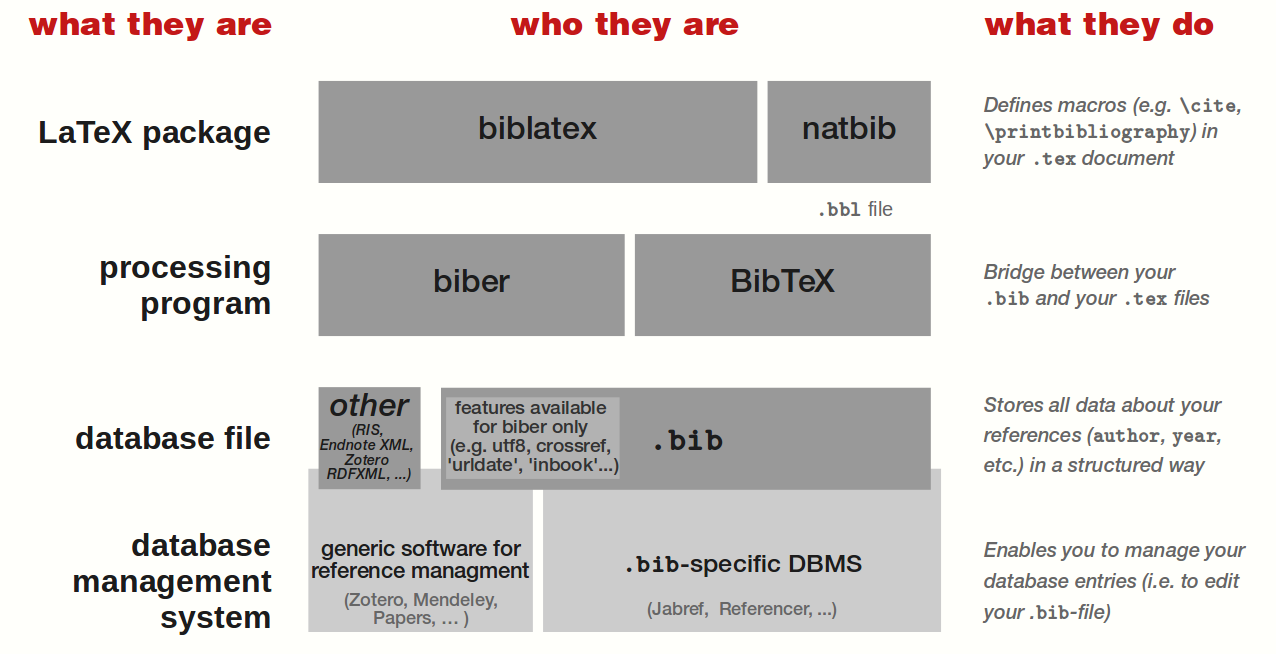
\includegraphics[width=0.8\textwidth]{content/citations_overview.png}
    \caption{Bibliography Process Overview in LaTeX}
    \label{fig: bibliography-process}
\end{figure}

At the highest level, there are two main front-end LaTeX packages that users interact with to handle citations, references, and bibliographies. These are \texttt{natbib} and \texttt{biblatex}. \texttt{natbib} is an older package, and although still maintained, may not be further developed. Despite this reasons, it is still widely used, and very reliable in nature. 
\texttt{biblatex} is a newer package that is more flexible and can handle more complex bibliography styles, and happens to be actively developed alongside the \texttt{biber} processing program (backend, more on this below). The humanities fields tend to use \texttt{biblatex} as many predefined styles are available (e.g., APA, MLA, Chicago). Science fields tend to go either way depending on the publishing journal's requirements and specific functionalities needed.

The backend or processing programs are the bridge between the LaTeX document and the bibliography file. The two main programs are \texttt{bibtex} and \texttt{biber}. \texttt{bibtex} interfaces with with specific \texttt{.bst} files, which are postfix language files that define the formatting of the bibliography. In the case of many major publication journals (especially in astronomy), the submission of manuscripts require the use of these \texttt{.bst} files, and as such, users are required to use the \texttt{natbib} LaTeX package. \texttt{biber} on the other hand is a relatively newer processing program that adds further functionality to \texttt{biblatex}.

It is important to note that the \texttt{biblatex} package can make use of either the \texttt{biber} backend or the \texttt{bibtex} backend, while the \texttt{natbib} package is restricted to the \texttt{bibtex} backend. Even more importantly, results with \texttt{biblatex} can differ depending on the backend: if \texttt{bibtex} is used, it only uses it for sorting, and not for formatting content.

The takeaways are the following: if you enjoy a particular style given in a particular journal, download it's \texttt{.bst} file and make use of the \texttt{natbib} package to compile your thesis work. In the case of this example PDF, the \texttt{aasjournal.bst} file is loaded, and it's style used in the bibliography:

\begin{lstlisting}[language=TeX]
    \TOCadd{Bibliography} % add citations to TOC
    \bibliography{AstroCitations.bib}{}
    \bibliographystyle{aasjournal} % links to aasjournal.bst file
\end{lstlisting}

A citation example is given here \citep{Hubble1929}.


    % see compiled PDF for information regarding citation styles
    \TOCadd{Bibliography} % add citations to TOC
    \bibliography{AstroCitations.bib}{}
    \bibliographystyle{aasjournal} % links to aasjournal.bst file

    % uncomment the following lines to include an appendix
    % \appendix
    % \include{content/appendix}

\end{document}
